%% AMS-LaTeX Created with the Wolfram Language : www.wolfram.com

\documentclass{article}
\usepackage{amsmath, amssymb, graphics, setspace}

\newcommand{\mathsym}[1]{{}}
\newcommand{\unicode}[1]{{}}

\newcounter{mathematicapage}
\begin{document}

\section*{$\unicode{0418}\unicode{043d}\unicode{0442}\unicode{0435}\unicode{0440}\unicode{043f}\unicode{043e}\unicode{043b}\unicode{044f}\unicode{0446}\unicode{0438}\unicode{044f}$
$\unicode{0444}\unicode{0443}\unicode{043d}\unicode{043a}\unicode{0446}\unicode{0438}\unicode{0438}$ \(f(x)=\frac{1}{\left(1+x^2\right)}\) $\unicode{043d}\unicode{0430}$
$\unicode{0440}\unicode{0430}\unicode{0432}\unicode{043d}\unicode{043e}\unicode{043c}\unicode{0435}\unicode{0440}\unicode{043d}\unicode{043e}\unicode{0439}$
$\unicode{0441}\unicode{0435}\unicode{0442}\unicode{043a}\unicode{0435}$}

$\unicode{0418}\unicode{0437}\unicode{043d}\unicode{0430}\unicode{0447}\unicode{0430}\unicode{043b}\unicode{044c}\unicode{043d}\unicode{0430}\unicode{044f}$
$\unicode{0444}\unicode{0443}\unicode{043d}\unicode{043a}\unicode{0446}\unicode{0438}\unicode{044f}$:

\begin{doublespace}
\noindent\(\pmb{f[\text{x$\_$}] = 1/(1+x{}^{\wedge}2);}\\
\pmb{\text{Plot}[f[x], \{x, -6, 6\}]}\)
\end{doublespace}

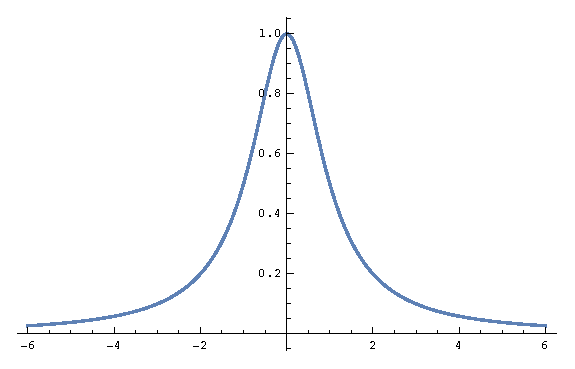
\includegraphics{report_gr1.eps}

$\unicode{0420}\unicode{0430}\unicode{0437}\unicode{043e}\unicode{0431}\unicode{044c}\unicode{0435}\unicode{043c}$ $\unicode{043f}\unicode{0440}\unicode{043e}\unicode{043c}\unicode{0435}\unicode{0436}\unicode{0443}\unicode{0442}\unicode{043e}\unicode{043a}$
$\unicode{043d}\unicode{0430}$ 4, 8, 16 $\unicode{0438}\unicode{043d}\unicode{0442}\unicode{0435}\unicode{0440}\unicode{0432}\unicode{0430}\unicode{043b}\unicode{043e}\unicode{0432}$:

\begin{doublespace}
\noindent\(\pmb{\text{data1} = N[f[\text{Range}[-6, 6,3]]]}\\
\pmb{\text{data2} = N[f[\text{Range}[-6, 6,1.5 ]]]}\\
\pmb{\text{data3} = N[f[\text{Range}[-6, 6,0.75 ]]]}\)
\end{doublespace}

\begin{doublespace}
\noindent\(\{0.027027,0.1,1.,0.1,0.027027\}\)
\end{doublespace}

\begin{doublespace}
\noindent\(\{0.027027,0.0470588,0.1,0.307692,1.,0.307692,0.1,0.0470588,0.027027\}\)
\end{doublespace}

\begin{doublespace}
\noindent\(\{0.027027,0.0350109,0.0470588,0.06639,0.1,0.164948,0.307692,0.64,1.,0.64,0.307692,0.164948,0.1,0.06639,0.0470588,0.0350109,0.027027\}\)
\end{doublespace}

$\unicode{0417}\unicode{0430}\unicode{043f}\unicode{0443}\unicode{0441}\unicode{0442}\unicode{0438}\unicode{043c}$ $\unicode{043f}\unicode{0440}\unicode{043e}\unicode{0433}\unicode{0440}\unicode{0430}\unicode{043c}\unicode{043c}\unicode{0443}$
$\unicode{0434}\unicode{043b}\unicode{044f}$ q = 200:

\begin{doublespace}
\noindent\(\pmb{\text{res1} = \text{Import}[\text{{``}/Users/severin/Desktop/$\unicode{041f}\unicode{0440}\unicode{0430}\unicode{043a}\unicode{0442}\unicode{0438}\unicode{043a}\unicode{0443}\unicode{043c}$/numerical-task-2.1/res$\_$uniform.dat{''}}];}\)
\end{doublespace}

\begin{doublespace}
\noindent\(\pmb{\text{res2} = \text{Import}[\text{{``}/Users/severin/Desktop/$\unicode{041f}\unicode{0440}\unicode{0430}\unicode{043a}\unicode{0442}\unicode{0438}\unicode{043a}\unicode{0443}\unicode{043c}$/numerical-task-2.1/res$\_$uniform.dat{''}}];}\)
\end{doublespace}

\begin{doublespace}
\noindent\(\pmb{\text{res3} = \text{Import}[\text{{``}/Users/severin/Desktop/$\unicode{041f}\unicode{0440}\unicode{0430}\unicode{043a}\unicode{0442}\unicode{0438}\unicode{043a}\unicode{0443}\unicode{043c}$/numerical-task-2.1/res$\_$uniform.dat{''}}];}\)
\end{doublespace}

$\unicode{041f}\unicode{043e}\unicode{0441}\unicode{0442}\unicode{0440}\unicode{043e}\unicode{0438}\unicode{043c}$ $\unicode{0433}\unicode{0440}\unicode{0430}\unicode{0444}\unicode{0438}\unicode{043a}\unicode{0438}$:

\begin{doublespace}
\noindent\(\pmb{\text{Show}[\text{Plot}[f[x], \{x, -6, 6\}, \text{ImageSize}\to \text{Medium}, \text{PlotStyle}\to \{\text{Red}\}],}\\
\pmb{\text{ListLinePlot}[\{\text{Transpose}@\{\text{Range}[-6, 6,12/800],\text{Drop}[\text{res1}, 2] \text{//.}\{\text{x$\_$}\}\text{:$>$}x\}, }\\
\pmb{\text{Transpose}@\{\text{Range}[-6, 6,12/1600], \text{Drop}[\text{res2}, 2] \text{//.}\{\text{x$\_$}\}\text{:$>$}x\}, }\\
\pmb{\text{Transpose}@\{\text{Range}[-6, 6,12/3200],\text{Drop}[\text{res3}, 2] \text{//.}\{\text{x$\_$}\}\text{:$>$}x\}\}, }\\
\pmb{\text{PlotStyle}\to \{\text{RGBColor}[0.8, 0.8, 0.8], \text{RGBColor}[0.7, 0.7, 0.7], \text{RGBColor}[0.6, 0.6, 0.6], }\\
\pmb{\text{RGBColor}[0.9, 0.9, 0.9]\}]]}\)
\end{doublespace}

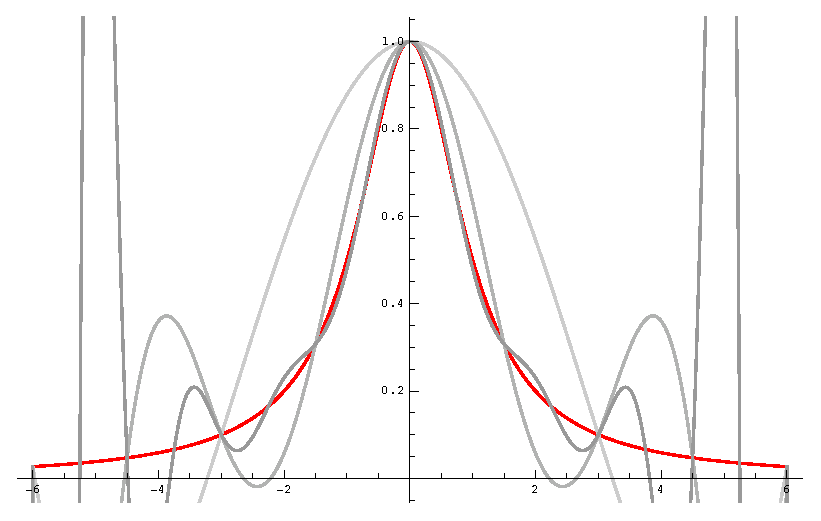
\includegraphics{report_gr2.eps}

$\unicode{0418}\unicode{0437}$ $\unicode{0433}\unicode{0440}\unicode{0430}\unicode{0444}\unicode{0438}\unicode{043a}\unicode{0430}$ $\unicode{0432}\unicode{0438}\unicode{0434}\unicode{043d}\unicode{043e}$,
$\unicode{0447}\unicode{0442}\unicode{043e}$ $\unicode{043f}\unicode{043e}\unicode{043b}\unicode{0443}\unicode{0447}\unicode{0430}\unicode{0435}\unicode{0442}\unicode{0441}\unicode{044f}$
$\unicode{0431}\unicode{0440}\unicode{0435}\unicode{0434}$.

\section*{$\unicode{0418}\unicode{043d}\unicode{0442}\unicode{0435}\unicode{0440}\unicode{043f}\unicode{043e}\unicode{043b}\unicode{044f}\unicode{0446}\unicode{0438}\unicode{044f}$
$\unicode{0444}\unicode{0443}\unicode{043d}\unicode{043a}\unicode{0446}\unicode{0438}\unicode{0438}$ \(f(x)=\frac{1}{\left(1+x^2\right)}\) $\unicode{043d}\unicode{0430}$
$\unicode{0427}\unicode{0435}\unicode{0431}\unicode{044b}\unicode{0448}\unicode{0435}\unicode{0432}\unicode{0441}\unicode{043a}\unicode{043e}\unicode{0439}$
$\unicode{0441}\unicode{0435}\unicode{0442}\unicode{043a}\unicode{0435}$}

$\unicode{0421}\unicode{043d}\unicode{043e}\unicode{0432}\unicode{0430}$ $\unicode{0440}\unicode{0430}\unicode{0437}\unicode{043e}\unicode{0431}\unicode{044c}\unicode{0435}\unicode{043c}$
$\unicode{043f}\unicode{0440}\unicode{043e}\unicode{043c}\unicode{0435}\unicode{0436}\unicode{0443}\unicode{0442}\unicode{043e}\unicode{043a}$ $\unicode{043d}\unicode{0430}$
4, 8, 16 $\unicode{0438}\unicode{043d}\unicode{0442}\unicode{0435}\unicode{0440}\unicode{0432}\unicode{0430}\unicode{043b}\unicode{043e}\unicode{0432}$,
$\unicode{043d}\unicode{0430}$ $\unicode{044d}\unicode{0442}\unicode{043e}\unicode{0442}$ $\unicode{0440}\unicode{0430}\unicode{0437}$ $\unicode{043f}\unicode{043e}$-$\unicode{0447}\unicode{0435}\unicode{0431}\unicode{044b}\unicode{0448}\unicode{0435}\unicode{0432}\unicode{0441}\unicode{043a}\unicode{0438}$:

\begin{doublespace}
\noindent\(\pmb{a = -6;}\\
\pmb{b = 6;}\\
\pmb{\text{cheb}[\text{k$\_$}, \text{n$\_$}] \text{:=}(a+b)/2.0+(a-b)/2.0*\text{Cos}[(2.0*k+1.0)/(2.0*n+2.0)*\text{Pi}]}\)
\end{doublespace}

\begin{doublespace}
\noindent\(\pmb{\text{data1} = N[f[\text{cheb}[\text{Range}[0, 4, 1],4]]]}\\
\pmb{\text{data2} = N[f[\text{cheb}[\text{Range}[0, 8, 1],8]]]}\\
\pmb{\text{data3} = N[f[\text{cheb}[\text{Range}[0, 16, 1],16]]]}\)
\end{doublespace}

\begin{doublespace}
\noindent\(\{0.0297953,0.0744175,1.,0.0744175,0.0297953\}\)
\end{doublespace}

\begin{doublespace}
\noindent\(\{0.0278439,0.0357143,0.0629948,0.191894,1.,0.191894,0.0629948,0.0357143,0.0278439\}\)
\end{doublespace}

\begin{doublespace}
\noindent\(\{0.0272528,0.0291512,0.0335037,0.0417957,0.0576729,0.091102,0.175505,0.451365,1.,0.451365,0.175505,0.091102,0.0576729,0.0417957,0.0335037,0.0291512,0.0272528\}\)
\end{doublespace}

$\unicode{0417}\unicode{0430}\unicode{043f}\unicode{0443}\unicode{0441}\unicode{0442}\unicode{0438}\unicode{043c}$ $\unicode{043f}\unicode{0440}\unicode{043e}\unicode{0433}\unicode{0440}\unicode{0430}\unicode{043c}\unicode{043c}\unicode{0443}$
$\unicode{0434}\unicode{043b}\unicode{044f}$ q = 200:

\begin{doublespace}
\noindent\(\pmb{\text{res1} = \text{Import}[\text{{``}/Users/severin/Desktop/$\unicode{041f}\unicode{0440}\unicode{0430}\unicode{043a}\unicode{0442}\unicode{0438}\unicode{043a}\unicode{0443}\unicode{043c}$/numerical-task-2.1/res$\_$chebyshev.dat{''}}];}\)
\end{doublespace}

\begin{doublespace}
\noindent\(\pmb{\text{res2} = \text{Import}[\text{{``}/Users/severin/Desktop/$\unicode{041f}\unicode{0440}\unicode{0430}\unicode{043a}\unicode{0442}\unicode{0438}\unicode{043a}\unicode{0443}\unicode{043c}$/numerical-task-2.1/res$\_$chebyshev.dat{''}}];}\)
\end{doublespace}

\begin{doublespace}
\noindent\(\pmb{\text{res3} = \text{Import}[\text{{``}/Users/severin/Desktop/$\unicode{041f}\unicode{0440}\unicode{0430}\unicode{043a}\unicode{0442}\unicode{0438}\unicode{043a}\unicode{0443}\unicode{043c}$/numerical-task-2.1/res$\_$chebyshev.dat{''}}];}\)
\end{doublespace}

$\unicode{041f}\unicode{043e}\unicode{0441}\unicode{0442}\unicode{0440}\unicode{043e}\unicode{0438}\unicode{043c}$ $\unicode{0433}\unicode{0440}\unicode{0430}\unicode{0444}\unicode{0438}\unicode{043a}\unicode{0438}$:

\begin{doublespace}
\noindent\(\pmb{\text{Show}[\text{Plot}[f[x], \{x, -6, 6\}, \text{ImageSize}\to \text{Medium}, \text{PlotStyle}\to \{\text{Red}\}],}\\
\pmb{\text{ListLinePlot}[\{\text{Transpose}@\{\text{Range}[-6, 6,12/800],\text{Drop}[\text{res1}, 2] \text{//.}\{\text{x$\_$}\}\text{:$>$}x\}, }\\
\pmb{\text{Transpose}@\{\text{Range}[-6, 6,12/1600], \text{Drop}[\text{res2}, 2] \text{//.}\{\text{x$\_$}\}\text{:$>$}x\}, }\\
\pmb{\text{Transpose}@\{\text{Range}[-6, 6,12/3200],\text{Drop}[\text{res3}, 2] \text{//.}\{\text{x$\_$}\}\text{:$>$}x\}\}, }\\
\pmb{\text{PlotStyle}\to \{\text{RGBColor}[0.8, 0.8, 0.8], \text{RGBColor}[0.7, 0.7, 0.7], \text{RGBColor}[0.6, 0.6, 0.6], }\\
\pmb{\text{RGBColor}[0.9, 0.9, 0.9]\}]]}\)
\end{doublespace}

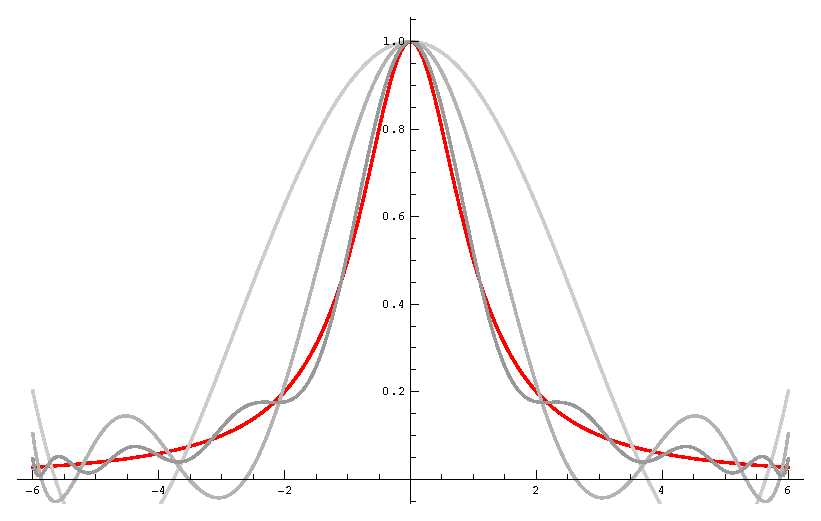
\includegraphics{report_gr3.eps}

$\unicode{042d}\unicode{0442}\unicode{043e}$ $\unicode{0443}\unicode{0436}\unicode{0435}$ $\unicode{043a}\unicode{0443}\unicode{0434}\unicode{0430}$
$\unicode{043b}\unicode{0443}\unicode{0447}\unicode{0448}\unicode{0435}$.

\section*{$\unicode{0418}\unicode{043d}\unicode{0442}\unicode{0435}\unicode{0440}\unicode{043f}\unicode{043e}\unicode{043b}\unicode{044f}\unicode{0446}\unicode{0438}\unicode{044f}$
$\unicode{043a}\unicode{043e}\unicode{043d}\unicode{0441}\unicode{0442}\unicode{0430}\unicode{043d}\unicode{0442}\unicode{043d}\unicode{043e}\unicode{0439}$
$\unicode{0444}\unicode{0443}\unicode{043d}\unicode{043a}\unicode{0446}\unicode{0438}\unicode{0438}$ $\unicode{043d}\unicode{0430}$ $\unicode{0440}\unicode{0430}\unicode{0432}\unicode{043d}\unicode{043e}\unicode{043c}\unicode{0435}\unicode{0440}\unicode{043d}\unicode{043e}\unicode{0439}$
$\unicode{0441}\unicode{0435}\unicode{0442}\unicode{043a}\unicode{0435}$}

$\unicode{0412}\unicode{043e}\unicode{0437}\unicode{044c}\unicode{043c}\unicode{0435}\unicode{043c}$ $\unicode{0441}\unicode{043b}\unicode{0435}\unicode{0434}\unicode{0443}\unicode{044e}\unicode{0449}\unicode{0438}\unicode{0435}$
$\unicode{0434}\unicode{0430}\unicode{043d}\unicode{043d}\unicode{044b}\unicode{0435}$:

\begin{doublespace}
\noindent\(\pmb{\text{data1} = \{0, 0, 1, 0, 0\};}\\
\pmb{\text{data2} = \{0, 0, 0, 0, 1, 0, 0, 0, 0\};}\\
\pmb{\text{data3} =\{0, 0, 0, 0, 0, 0, 0, 0, 1, 0, 0, 0, 0, 0, 0, 0, 0\};}\)
\end{doublespace}

$\unicode{0417}\unicode{0430}\unicode{043f}\unicode{0443}\unicode{0441}\unicode{0442}\unicode{0438}\unicode{043c}$ $\unicode{043f}\unicode{0440}\unicode{043e}\unicode{0433}\unicode{0440}\unicode{0430}\unicode{043c}\unicode{043c}\unicode{0443}$
$\unicode{0434}\unicode{043b}\unicode{044f}$ q = 200:

\begin{doublespace}
\noindent\(\pmb{\text{res1} = \text{Import}[\text{{``}/Users/severin/Desktop/$\unicode{041f}\unicode{0440}\unicode{0430}\unicode{043a}\unicode{0442}\unicode{0438}\unicode{043a}\unicode{0443}\unicode{043c}$/numerical-task-2.1/res$\_$uniform.dat{''}}];}\)
\end{doublespace}

\begin{doublespace}
\noindent\(\pmb{\text{res2} = \text{Import}[\text{{``}/Users/severin/Desktop/$\unicode{041f}\unicode{0440}\unicode{0430}\unicode{043a}\unicode{0442}\unicode{0438}\unicode{043a}\unicode{0443}\unicode{043c}$/numerical-task-2.1/res$\_$uniform.dat{''}}];}\)
\end{doublespace}

\begin{doublespace}
\noindent\(\pmb{\text{res3} = \text{Import}[\text{{``}/Users/severin/Desktop/$\unicode{041f}\unicode{0440}\unicode{0430}\unicode{043a}\unicode{0442}\unicode{0438}\unicode{043a}\unicode{0443}\unicode{043c}$/numerical-task-2.1/res$\_$uniform.dat{''}}];}\)
\end{doublespace}

$\unicode{041f}\unicode{043e}\unicode{0441}\unicode{0442}\unicode{0440}\unicode{043e}\unicode{0438}\unicode{043c}$ $\unicode{0433}\unicode{0440}\unicode{0430}\unicode{0444}\unicode{0438}\unicode{043a}\unicode{0438}$:

\begin{doublespace}
\noindent\(\pmb{\text{Show}[\text{ListLinePlot}[\{\text{Transpose}@\{\text{Range}[-6, 6,12/800],\text{Drop}[\text{res1}, 2] \text{//.}\{\text{x$\_$}\}\text{:$>$}x\},
}\\
\pmb{\text{Transpose}@\{\text{Range}[-6, 6,12/1600], \text{Drop}[\text{res2}, 2] \text{//.}\{\text{x$\_$}\}\text{:$>$}x\}, }\\
\pmb{\text{Transpose}@\{\text{Range}[-6, 6,12/3200],\text{Drop}[\text{res3}, 2] \text{//.}\{\text{x$\_$}\}\text{:$>$}x\}\}, }\\
\pmb{\text{PlotStyle}\to \{\text{RGBColor}[0.8, 0.8, 0.8], \text{RGBColor}[0.7, 0.7, 0.7], \text{RGBColor}[0.6, 0.6, 0.6], }\\
\pmb{\text{RGBColor}[0.9, 0.9, 0.9]\}]]}\)
\end{doublespace}

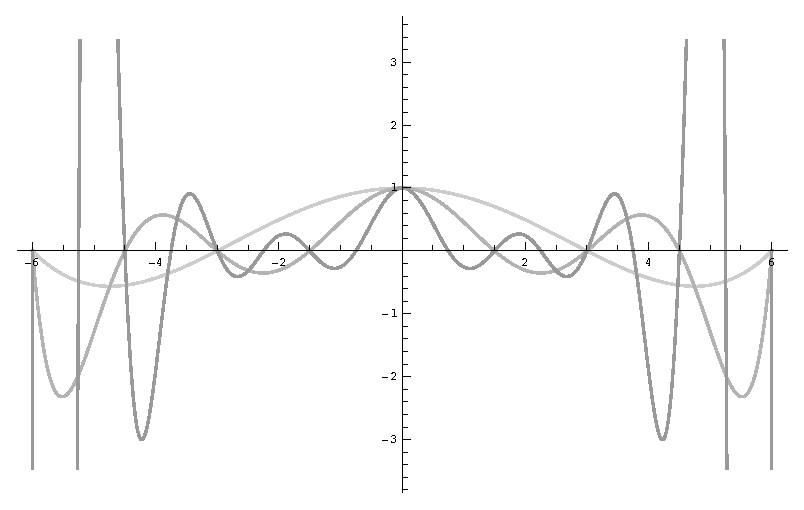
\includegraphics{report_gr4.eps}

$\unicode{041f}\unicode{043b}\unicode{043e}\unicode{0445}\unicode{043e}$ $\unicode{043f}\unicode{043e}\unicode{043b}\unicode{0443}\unicode{0447}\unicode{0438}\unicode{043b}\unicode{043e}\unicode{0441}\unicode{044c}$.

\section*{$\unicode{0418}\unicode{043d}\unicode{0442}\unicode{0435}\unicode{0440}\unicode{043f}\unicode{043e}\unicode{043b}\unicode{044f}\unicode{0446}\unicode{0438}\unicode{044f}$
$\unicode{043a}\unicode{043e}\unicode{043d}\unicode{0441}\unicode{0442}\unicode{0430}\unicode{043d}\unicode{0442}\unicode{043d}\unicode{043e}\unicode{0439}$
$\unicode{0444}\unicode{0443}\unicode{043d}\unicode{043a}\unicode{0446}\unicode{0438}\unicode{0438}$ $\unicode{043d}\unicode{0430}$ $\unicode{0427}\unicode{0435}\unicode{0431}\unicode{044b}\unicode{0448}\unicode{0435}\unicode{0432}\unicode{0441}\unicode{043a}\unicode{043e}\unicode{0439}$
$\unicode{0441}\unicode{0435}\unicode{0442}\unicode{043a}\unicode{0435}$}

$\unicode{041f}\unicode{043e}$ $\unicode{0430}\unicode{043d}\unicode{0430}\unicode{043b}\unicode{043e}\unicode{0433}\unicode{0438}\unicode{0447}\unicode{043d}\unicode{044b}\unicode{043c}$
$\unicode{0434}\unicode{0430}\unicode{043d}\unicode{043d}\unicode{044b}\unicode{043c}$ $\unicode{0437}\unicode{0430}\unicode{043f}\unicode{0443}\unicode{0441}\unicode{0442}\unicode{0438}\unicode{043c}$
$\unicode{043f}\unicode{0440}\unicode{043e}\unicode{0433}\unicode{0440}\unicode{0430}\unicode{043c}\unicode{043c}\unicode{0443}$ $\unicode{0434}\unicode{043b}\unicode{044f}$
q = 200:

\begin{doublespace}
\noindent\(\pmb{\text{res1} = \text{Import}[\text{{``}/Users/severin/Desktop/$\unicode{041f}\unicode{0440}\unicode{0430}\unicode{043a}\unicode{0442}\unicode{0438}\unicode{043a}\unicode{0443}\unicode{043c}$/numerical-task-2.1/res$\_$chebyshev.dat{''}}];}\)
\end{doublespace}

\begin{doublespace}
\noindent\(\pmb{\text{res2} = \text{Import}[\text{{``}/Users/severin/Desktop/$\unicode{041f}\unicode{0440}\unicode{0430}\unicode{043a}\unicode{0442}\unicode{0438}\unicode{043a}\unicode{0443}\unicode{043c}$/numerical-task-2.1/res$\_$chebyshev.dat{''}}];}\)
\end{doublespace}

\begin{doublespace}
\noindent\(\pmb{\text{res3} = \text{Import}[\text{{``}/Users/severin/Desktop/$\unicode{041f}\unicode{0440}\unicode{0430}\unicode{043a}\unicode{0442}\unicode{0438}\unicode{043a}\unicode{0443}\unicode{043c}$/numerical-task-2.1/res$\_$chebyshev.dat{''}}];}\)
\end{doublespace}

$\unicode{041f}\unicode{043e}\unicode{0441}\unicode{0442}\unicode{0440}\unicode{043e}\unicode{0438}\unicode{043c}$ $\unicode{0433}\unicode{0440}\unicode{0430}\unicode{0444}\unicode{0438}\unicode{043a}\unicode{0438}$:

\begin{doublespace}
\noindent\(\pmb{\text{Show}[\text{ListLinePlot}[\{\text{Transpose}@\{\text{Range}[-6, 6,12/800],\text{Drop}[\text{res1}, 2] \text{//.}\{\text{x$\_$}\}\text{:$>$}x\},
}\\
\pmb{\text{Transpose}@\{\text{Range}[-6, 6,12/1600], \text{Drop}[\text{res2}, 2] \text{//.}\{\text{x$\_$}\}\text{:$>$}x\}, }\\
\pmb{\text{Transpose}@\{\text{Range}[-6, 6,12/3200],\text{Drop}[\text{res3}, 2] \text{//.}\{\text{x$\_$}\}\text{:$>$}x\}\}, }\\
\pmb{\text{PlotStyle}\to \{\text{RGBColor}[0.8, 0.8, 0.8], \text{RGBColor}[0.7, 0.7, 0.7], \text{RGBColor}[0.6, 0.6, 0.6], }\\
\pmb{\text{RGBColor}[0.9, 0.9, 0.9]\}]]}\)
\end{doublespace}

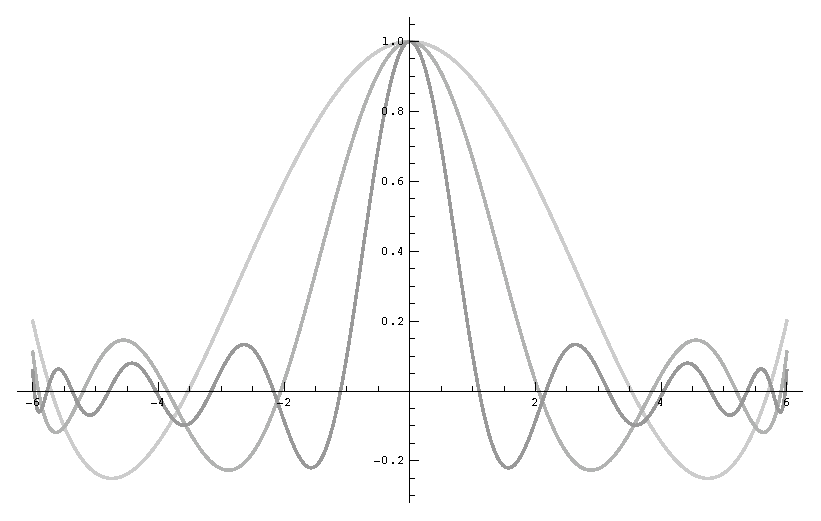
\includegraphics{report_gr5.eps}

$\unicode{0421}\unicode{043d}\unicode{043e}\unicode{0432}\unicode{0430}$ $\unicode{043b}\unicode{0443}\unicode{0447}\unicode{0448}\unicode{0435}$.

\section*{$\unicode{0412}\unicode{044b}\unicode{0432}\unicode{043e}\unicode{0434}$ $---$ $\unicode{0438}\unicode{043d}\unicode{0442}\unicode{0435}\unicode{0440}\unicode{043f}\unicode{043e}\unicode{043b}\unicode{044f}\unicode{0446}\unicode{0438}\unicode{044f}$
$\unicode{043f}\unicode{043e}$ $\unicode{0427}\unicode{0435}\unicode{0431}\unicode{044b}\unicode{0448}\unicode{0435}\unicode{0432}\unicode{0443}$
$\unicode{0442}\unicode{043e}\unicode{0447}\unicode{043d}\unicode{0435}\unicode{0435}$, $\unicode{0445}\unicode{043e}\unicode{0442}\unicode{044c}$
$\unicode{0438}$ $\unicode{0442}\unicode{0440}\unicode{0435}\unicode{0431}\unicode{0443}\unicode{0435}\unicode{0442}$ 5 $\unicode{0432}\unicode{043b}\unicode{043e}\unicode{0436}\unicode{0435}\unicode{043d}\unicode{043d}\unicode{044b}\unicode{0445}$
$\unicode{0446}\unicode{0438}\unicode{043a}\unicode{043b}\unicode{043e}\unicode{0432}$ $\unicode{0432}\unicode{043c}\unicode{0435}\unicode{0441}\unicode{0442}\unicode{043e}$
3.}

\end{document}
